\documentclass[12pt,a4paper]{article}

\setcounter{tocdepth}{3}
\setcounter{secnumdepth}{2}

\usepackage[english]{babel}
\usepackage[utf8x]{inputenc}
\usepackage{amsmath}
\usepackage{amssymb}
\DeclareMathOperator*{\argmin}{arg\,min}
\usepackage{graphicx}
\usepackage{etoolbox}
\usepackage[nottoc]{tocbibind}
\usepackage[toc,page]{appendix}
\usepackage{cite}
\usepackage[]{program}
\usepackage{algorithm}
\usepackage[noend]{algpseudocode}
\usepackage{array}
\usepackage{indentfirst}
\usepackage{chngcntr}

\usepackage{version}

\makeatletter
\def\BState{\State\hskip-\ALG@thistlm}
\makeatother
\usepackage{chngcntr}

\newtheorem{definition}{Definition}
\newtheorem{theorem}{Theorem}

\begin{document}

%----------------------------------------------------------------------------------------
%	TITLE PAGE
%----------------------------------------------------------------------------------------

\begin{titlepage}
	\centering
	
\includegraphics[width=0.15\textwidth]{ensae.jpg}\par\vspace{1cm}
	{\scshape\LARGE ENSAE ParisTech\par}
	\vspace{1cm}
	{\scshape\Large Master 1st year Python Machine Learning Project\par}
	\vspace{1.5cm}
	{\huge\bfseries On-Policy Reinforcement Learning for Blackjack\par}
	\vspace{2cm}
	{\Large\itshape by Mehdi Abbana Bennani\par}
	\vfill
	supervised by\par
	Pr.~Xavier \textsc{Dupré}\par    
	\vfill

% Bottom of the page
	{\large \today\par}
\end{titlepage}


%----------------------------------------------------------------------------------------
%	Abstract PAGE
%----------------------------------------------------------------------------------------

\newpage

\begin{abstract}

Reinforcement Learning is a major Machine Learning class of algorithms. In this report, I will apply some major RL algorithms to a simplified blackjack game, mostly inspired form the Easy21 Assignment by Prof. David Silver at UCL. I will demonstrate through simulations that these algorithms achieve a good performance in this framework.

\end{abstract}

%----------------------------------------------------------------------------------------
%	Contents PAGE
%----------------------------------------------------------------------------------------

\newpage
\tableofcontents

%----------------------------------------------------------------------------------------
%	Introduction PAGE
%----------------------------------------------------------------------------------------

\newpage

\section*{Introduction}
\addcontentsline{toc}{section}{Introduction}

The report is organized as follows:in the first part, I define the problem, in the second part I describe the reinforcement learning terminology and the algorithms I will use. In the third part, I will describe some important coding aspects such as code structure and performance improvement tricks.

\section*{Motivation}
\addcontentsline{toc}{section}{Motivation}
Reinforcement learning is a one of the major Machine Learning classes of algorithms. It achieved a better performance than many state of the art algorithms in many domains, such as in games\cite{mnih-dqn-2015}\cite{44806}, shape recognition\cite{DBLP:journals/corr/RezendeEMBJH16}, and it is used for some very complex problems such as driveless cars.

Through this assignment, I aim to:
\begin{itemize}
\item explore and understand Reinforcement Learning Algorithms
\item apply these algorithms to concrete problems and explore their limits
\item test new approaches and personal ideas in these problems
 \end{itemize}

\section*{Running the simulations}
The code can be retrieved under my GitHub repository :

https://github.com/MehdiAB161/Reinforcement-Learning.git
\\The running instructions are provided within the Readme file


%----------------------------------------------------------------------------------------
%	Problem definition Chapter
%----------------------------------------------------------------------------------------

\newpage
\section{Problem definition}

\subsection{Simple case}
This exercise is similar to the Blackjack
example in Sutton and Barto 5.3, however, the rules of the
card game are different and non-standard.
\begin{itemize}
\item The game is played with an infinite deck of cards (i.e. cards are sampled
with replacement). Each draw from the deck results in a value between 1 and 10 (uniformly
distributed) with a colour of red (probability 1/3) or black (probability
2/3). There are no aces or picture (face) cards in this game
\item At the start of the game both the player and the dealer draw one black
card (fully observed)
\item Each turn the player may either stick or hit. If the player hits then she draws another card from the deck. If the player sticks she receives no further cards
\item The values of the player’s cards are added (black cards) or subtracted (red
cards). If the player’s sum exceeds 51, or becomes less than 1, then she “goes
bust” and loses the game (reward -1)
\item If the player sticks then the dealer starts taking turns. The dealer always
sticks on any sum of 47 or greater, and hits otherwise. If the dealer goes
bust, then the player wins; otherwise, the outcome – win (reward +1),
lose (reward -1), or draw (reward 0) – is the player with the largest sum
\end{itemize}
 
\subsection{Card history memory integration and card sampling without replacement}
In this part, I will put additional constraints and drop some other hypotheses on the environment and the agent: 
 
\begin{itemize}
\item The cards sampling is without replacement, so there is a set of 30 cards, 20 black and 10 red, sampled with the same probability.
\item The agent will remember the cards which were played before and will adapt his actions to these information.
\item The dealer will not take into account this history and will play as defined in the previous section.
\end{itemize}
%----------------------------------------------------------------------------------------
%	Introduction
%----------------------------------------------------------------------------------------
\newpage

\section{Forumlation of Reinforcement Learning Problem}

\subsection{Definitions}

\begin{definition}{State Value Function}

The state value function v(s) of a Markov Reward Process is the expected return starting from state s

\[ 
v(s) = \mathbb{E}[G_{t} \vert S_{t}=s]
\]
\end{definition}

\begin{definition}{Policy}

A policy $\pi$ is a distribution over actions given states
\[ 
\pi(a\vert s) = \mathbb{P}[A_{t}=a \vert S_{t}=s]
\]
\end{definition}

\begin{definition}{Return}

The return $G_{t}$ is the total discounted reward from time step t.
\[ 
G_{t} = \sum_{k=0}^{\infty}{\gamma^{k}R_{t+k+1}}
\]
\end{definition}

\begin{definition}{State Value Function}

The state value function $v_{\pi}(s)$ of a MDP is the expected return starting from state s, and then following the policy $\pi$
\[ 
v_{\pi}(s) = \mathbb{E}[G_{t} \vert S_{t}=s]
\]
\end{definition}

\begin{definition}{State Action Value Function}

The state action value function $q_{\pi}(s, a)$ of a MDP is the expected return starting from state s, and taking action a, then following the policy $\pi$
\[ 
v_{\pi}(s) = \mathbb{E}[G_{t} \vert S_{t}=s]
\]

The state action value function $q_{\pi}(s, a)$ of a MDP is the expected return starting from state s, and taking action a, then following the policy $\pi$
\[ 
q_{\pi}(s) = \mathbb{E}[G_{t} \vert S_{t}=s, A_{t}=a]
\]

\end{definition}

\begin{definition}{Optimal Value Function}

The optimal state value function $v_{\star}(s)$ is the maximum state action value function over all policies
\[ 
v_{\star}(s) = \underset{\pi}{max}{v_{\pi}(s)}
\]

The optimal state action value function $q_{\star}(s, a)$ is the maximum state action value function over all policies
\[ 
q_{\star}(s, a) = \underset{\pi}{max}{q_{\pi}(s, a)}
\]
\end{definition}

\begin{definition}{Optimal Policy}

We define a partial ordering over a policies:

$\pi \geq \pi^{\prime}$ if $v_{\pi}(s) \geq  v_{\pi}(s)$

\end{definition}

\subsection{Theorems}

\begin{theorem}{Optimal Policy}
For any MDP
\begin{itemize}
\item There exists an optimal policy $\pi_{\star}$ that is better than or equal to all other policies $\pi_{\star} \geq \pi,\forall\pi $
\item All policies achieve the optimal value function $v_{\pi_{\star}} = v_{\star}$
\item All policies achieve the optimal state action value function $q_{\pi_{\star}} = q_{\star}$
\end{itemize}
\end{theorem}

\begin{theorem}{The Bellman Expectation Equation}

The state-value function can be decomposed into immediate reward plus discounted value of the successor state.
\[ 
v_{\pi}(s) = \mathbb{E}[R_{t+1} + \gamma v_{\pi}(S_{t+1})  \vert S_{t}=s]
\]

The action-value function can similarly be decomposed
\[ 
q_{\pi}(s) = \mathbb{E}[R_{t+1} + \gamma q_{\pi}(S_{t+1}, A_{t+1}) \vert S_{t}=s, A_{t}=a]
\]


\end{theorem}

\subsection{Monte Carlo Algorithms}

The intuition behind this algorithm is that, in order to estimate the value of a state action pair, we run a full episode, with a policy such as $\epsilon$ greedy policy,then we update our current estimation of the action-value function in the direction of the average of the action value estimation of all visited state-action pairs during the episode.

\begin{algorithm}
\caption{Greedy in the Limit with Infinite Exploration Algorithm (GLIE)}
\label{alg:glie}
\begin{algorithmic}[1]
\State Sample kth episode using $\pi: \left\{S_{1}, A_{1}, R_{1}, S_{2}, ...\right\}$
\For{$each state S_{t} and Action A_{t} in the episode$}
\State $N(S_{t}, A_{t}) \leftarrow N(S_{t}, A_{t}) + 1$
\State $Q(S_{t}, A_{t}) \leftarrow Q(S_{t}, A_{t}) + \frac{G_{t} - Q(S_{t}, A_{t})}{N(S_{t}, A_{t})}$
\EndFor
\State Improve policy based on new action-value function
\\ $\epsilon = 1/k $
\\ $\pi \Leftarrow \epsilon-greedy(Q) $
\end{algorithmic}
\end{algorithm}



\subsection{Temporal Difference Learning Algorithms}
\subsubsection{SARSA Algorithm}


The intuition behind this algorithm is that, in order to estimate the value of a state action pair, we run a full episode, with a policy such as $\epsilon$ greedy policy,then we update our current estimation of the action-value function in the direction of the average of the action value estimation of all visited state-action pairs during the episode.


\begin{algorithm}
\caption{SARSA Algorithm for On-Policy Control}
\label{alg:sarsa}
\begin{algorithmic}[1]
\State Initialize $Q(s,a),\forall s \in \mathbb{S}, a \in \mathbb{A}(s)$, arbitrarlily, and Q(terminal-state,-)=0
\For{each episode}
\State Initialize S
\State Choose A from S using policy derived from Q (e.g., $epsilon-greedy$)
\For{each step in the episode}
\State Take action A, observe R, $S^{\prime}$
\State Choose $A^{\prime}$ from $S^{\prime}$
\State $Q(S,A) \leftarrow Q(S,A) + \alpha(R + \gamma Q(S^{\prime}, A^{\prime}) - Q(S, A)$
\State $S \leftarrow S^{\prime}$
\State $A \leftarrow A^{\prime}$
\EndFor
\EndFor
\end{algorithmic}
\end{algorithm}

\subsubsection{SARSA-$\lambda$ Algorithm}

\begin{algorithm}
\caption{SARSA-$\lambda$ Algorithm for On-Policy Control}
\label{alg:sarsa_lambda}
\begin{algorithmic}[1]
\State Initialize $Q(s,a),\forall s \in \mathbb{S}, a \in \mathbb{A}(s)$, arbitrarily, and Q(terminal-state,-)=0
\For{each episode}
\State E(s,a) = 0 for all $s\in\mathbb{S}, a\in\mathbb{A}(s)$
\State Initialize S, A
\For{each step in the episode}
\State Take action A, observe R, $S^{\prime}$
\State Choose $A^{\prime}$ from $S^{\prime}$ using policy derived from Q (e.g. $\epsilon$greedy)
\State $\delta \leftarrow R + \gamma Q(S^{\prime},A^{\prime}) - Q(S,A) $
\State $E(S,A) \leftarrow E(S,A) + 1$ 
\For{all $s\in S, a \in \mathbf{A}(s) $}
\State $Q(s,a) \Leftarrow Q(s,a) + \alpha\delta E(s,a)$
\State $E(s,a) \leftarrow \gamma \lambda E(s,a)$
\EndFor
\State $A \leftarrow A^{\prime}, S \leftarrow S^{\prime},$
\EndFor
\EndFor
\end{algorithmic}
\end{algorithm}


\subsection{Action Value Function Approximation}
Where the state action space size is very big, we cannot use table lookup anymore to get the state action value function values for all states. In this case, we approximate the value function by parametrizing it.
The state action value function becomes $Q(S, A, w)$, where w is a vector which size is the feature space size.

In this case, we update the parameters w instead of updating every single state action pair value function. This approach also has some upsides such as approximating the value of state-actions that may be never visited.

In case of the Monte Carlo 'GLIE' algorithm, we operate the following update:

$\Delta w=\alpha (G_{t} - \hat{q}(S_{t}, A_{t}, w) )\nabla_{w}\hat{q}(S_{t}, A_{t}, w) )$ 

This equation means that we make a step in direction of the difference of our estimate and the sampled value with Monte Carlo.

For TD$-\lambda$, the update is as follows:

$\Delta w=\alpha (R_{t+1} + \gamma \hat{q}(S_{t+1}, A_{t+1}, w) ) - \hat{q}(S_{t}, A_{t}, w) )\nabla_{w}\hat{q}(S_{t}, A_{t}, w) )$ 


This equation means that we make a step in direction of the difference of our estimate and the sampled value with Sarsa $\lambda$.

\section{Reinforcement Learning applied to Blackjack}

\subsection{Experimental results}


I applied the Algorithms above to the simplified blackjack game defined in the first section.

I expect the Monte Carlo estimation to be the most stable algorithm, and is unbiased asymptotically.

I infered the state value function from the state action value function as the the value of the action which brings the most  value from state s $V(s,a) = argmaxQ(s,a)$  The results are shown in the figure ... In this figure, we can see that we can identify the mechanisms of the game. The value function is decreasing with the card value of the dealer. Also the value 10 is relatively safe for the player because he is sure not to lose the game, from 17 to 21 .........

The figure ... shows the value function using Sarsa lambda, in this figure we see that our estimate is more noisy than in the previous one. The reason is that Sarsa lambda is based on bootstrapping, therefore our updates are biased. I also expected Sarsa lambda to be slower in term of convergence speed, we can see that on the rmse figure.

For this application, value function approximation is not relevant because the state space is very small the size is equal to scoreLimit * 10, which in our case corresponds to 520 states. The chosen features' space size is ....  

First, I used linear function approximation, which I have theoretical convergence guaranties The result is displayed in figure ...
We can see that 

The RMSE is 

The other function approximation I used is quadratic approximation, I don't have theoretical convergence guaranties. The results are displayed in ....




\begin{figure}[!ht]
   \caption{\label{E21_MC_V} Optimal Value Function after 10⁶ episodes using GLIE}
   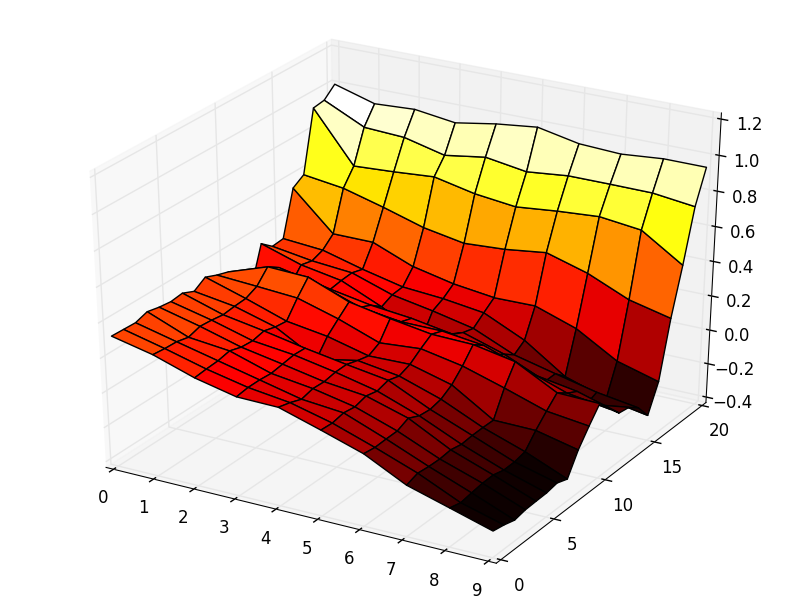
\includegraphics[scale=0.4]{Easy21_Results/MC_value_1e6.png}
\end{figure}

\begin{figure}[!ht]
   \caption{\label{E21_MC_D} Optimal Actions after 10⁶ episodes using GLIE}
   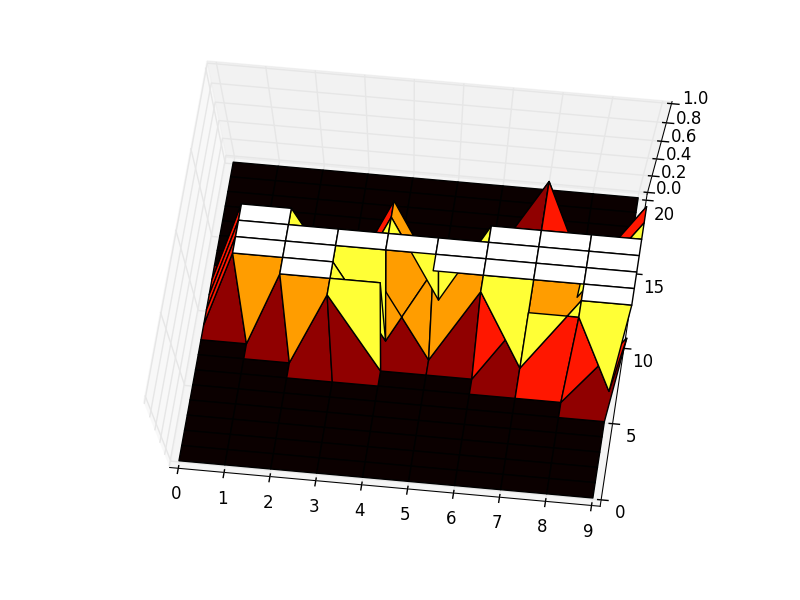
\includegraphics[scale=0.4]{Easy21_Results/MC_decision_1e6.png}
\end{figure}


\begin{figure}[!ht]
   \caption{\label{E21_S_V} Optimal Value Function after 10⁶ episodes using SARSA}
   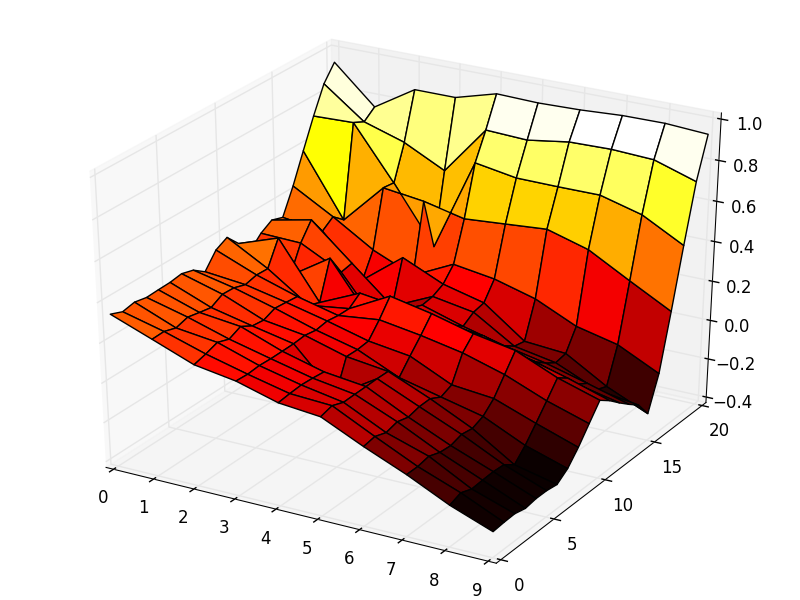
\includegraphics[scale=0.4]{Easy21_Results/Sarsa_value_1e6.png}
\end{figure}

\begin{figure}[!ht]
   \caption{\label{E21_S_D} Optimal Actions after 10⁶ episodes using SARSA}
   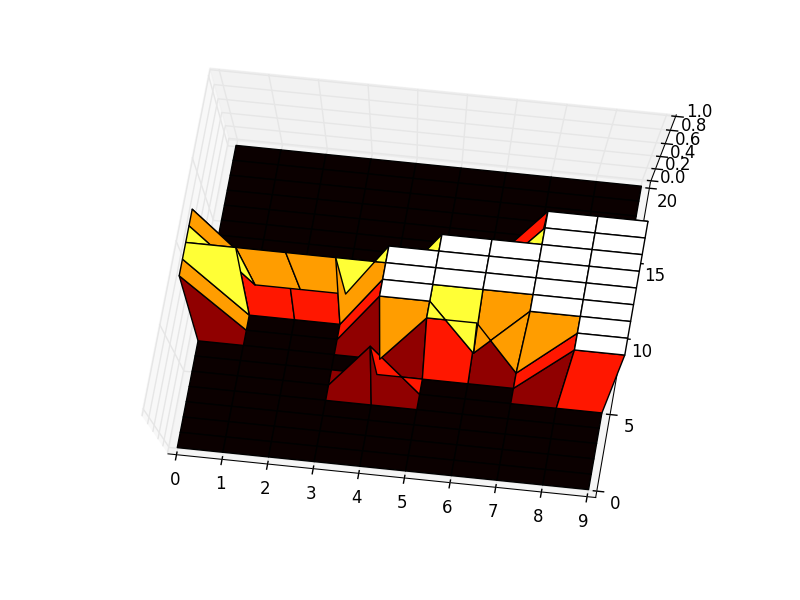
\includegraphics[scale=0.4]{Easy21_Results/Sarsa_decision_1e6.png}
\end{figure}


\begin{figure}[!ht]
   \caption{\label{E21_SL_V} Optimal Value Function after 10⁶ episodes using SARSA-$\lambda$ for $\lambda=0.8$}
   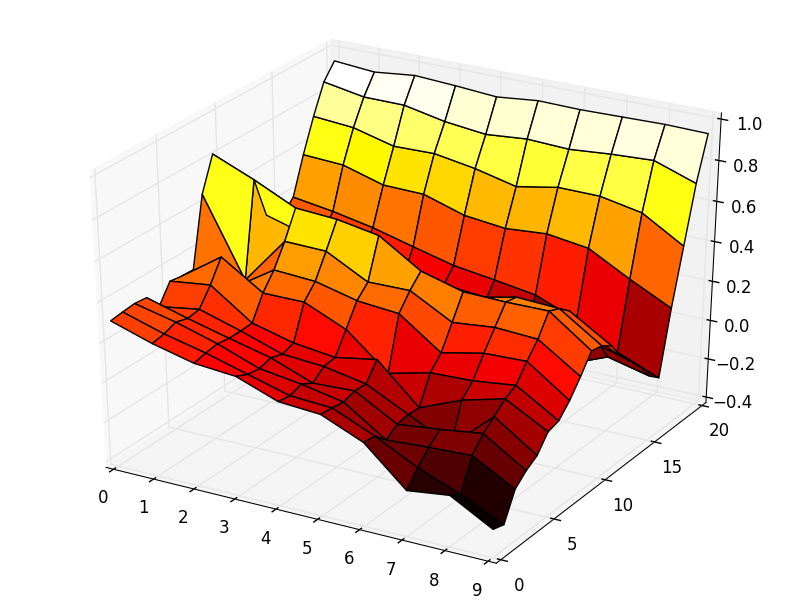
\includegraphics[scale=0.4]{Easy21_Results/Sarsa_lambda_0_8_value_1e6.png}
\end{figure}

\begin{figure}[!ht]
   \caption{\label{E21_SL_D} Optimal Actions after 10⁶ episodes using SARSA-$\lambda$ for $\lambda=0.8$}
   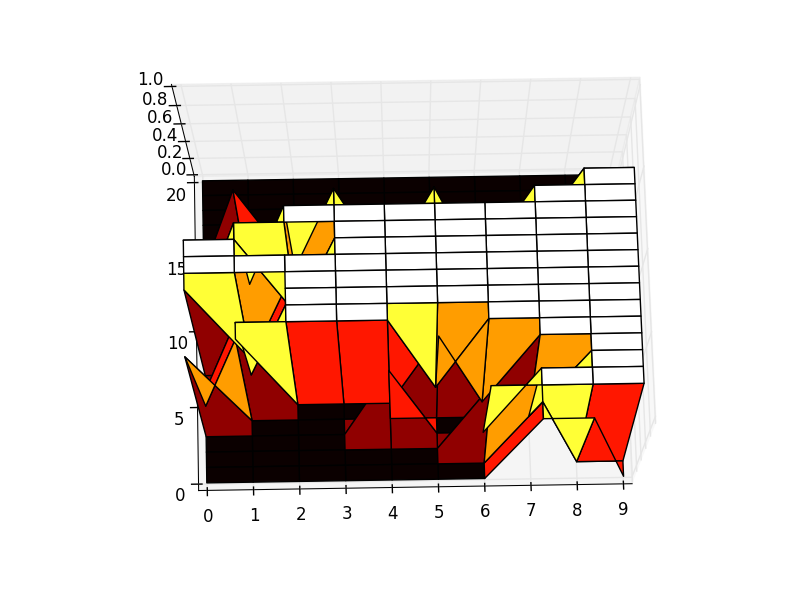
\includegraphics[scale=0.4]{Easy21_Results/Sarsa_lambda_0_8_decision_1e6.png}
\end{figure}

\begin{figure}[!ht]
   \caption{\label{E21_SL_LA_V} Optimal Value Function after 10⁶ episodes using Linear Function Approximation and SARSA-$\lambda$ for $\lambda=0.8$}
   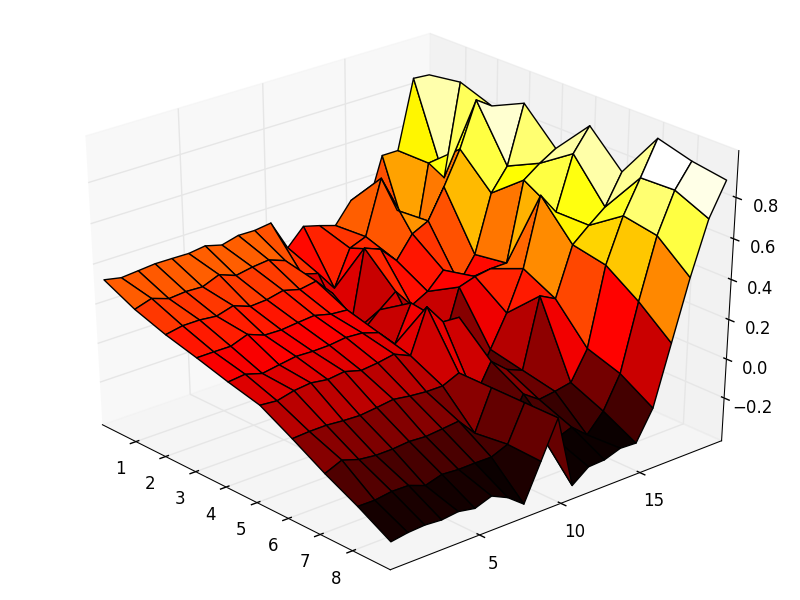
\includegraphics[scale=0.4]{Easy21_Results/Sarsa_0_8_linear_app_value_1e6.png}
\end{figure}

\begin{figure}[!ht]
   \caption{\label{E21_SL_LA_D} Optimal Value Function after 10⁶ episodes using Linear Function Approximation and SARSA-$\lambda$ for $\lambda=0.8$}
   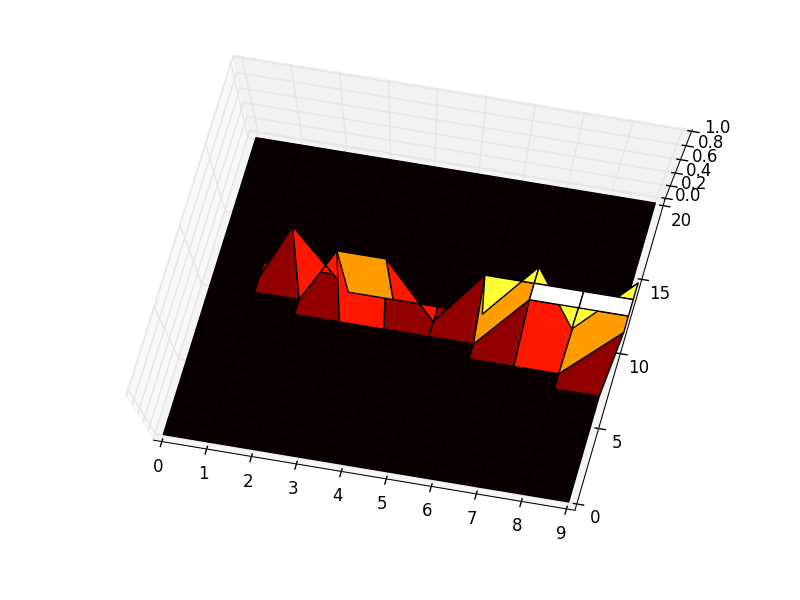
\includegraphics[scale=0.4]{Easy21_Results/Sarsa_0_8_linear_app_decision_1e6.png}
\end{figure}

\subsection{Further analysis}
In case of a very high dimensional state space, for example a finite card set without re-sampling and by integrating a memory to the agent. For 
It is not possible to use table lookup, therefore the basic Monte Caro GLIE and Temporal difference algorithms are intractable. State Action value function approximation is necessary. 

In case of 

\section{Conclusion and further possible developpements}
Deep Q Networks and Experience Replay \cite{mnih-dqn-2015}


%----------------------------------------------------------------------------------------
%	Bibliography
%----------------------------------------------------------------------------------------
\newpage
\nocite{*}
\bibliographystyle{plain}
\bibliography{bibliography}


\end{document}